\section{Introduction}
\begin{displayquote}
\textit{\textbf{\Huge{``}}
\large{Around 10\% of enterprise-generated data is created and processed outside a traditional centralized data center or cloud. By 2025, Gartner predicts this figure will reach 75\%.\cite{gartnerEdgeComputing:online}}
\textbf{\Huge{''}}}
\\[1pt]
\raggedleft{{\rm --- Gartner}}
\end{displayquote}
Data has never been as ubiquitous as it is today. Not only do our mobile phones constantly generate data but also the things we wear, use and own are now generating data. Not only the private sector is effected by this data revolution also the industry is embracing new technologies to gather data to automate processes. Some factories are even operated entirely self-sufficient without any human intervention. These factories are called "lights-out factories" and are becoming more and more popular\cite{wheresmyRobotLightsOut33:online}. In a world where data is everywhere the computing power to process this data has to be everywhere as well. Relying solemnly on centralized servers will eventually topple the system. The estimate by Gartner that 75\% of data will be generated and processed outside traditional data centers clearly shows decentralized architectures are here to stay.

In a curated report from the economist in 2015 the authors conclude that "cloud computing has the potential to disrupt entire industries, reshape businesses and markets and change the way we think about information"\cite{PuttogetEconomistCloud13:online}. Much of this success can be attributed to Kubernetes. It is a platform for container orchestration and was donated by Google to the open source community in 2014\cite{WhatisKubernetes87:online}. It enables the abstraction of hardware from deployments and provides much of the simplicity of Platform as a Service (Paas)\cite{WhatisKubernetes87:online}.

Edge computing is the term used for processing and storing data on the edge of the network. Fog computing is a subform of edge computing where the edge part is tightly integrated with the cloud to enhance both systems. This brings new possibilities and challenges to system designers.

{\LARGE{insert figure of simple edge setup here}}

In this thesis I will develop an exemplary fog system to remotely monitor and control lights. It is meant to show the areas Kubernetes excels in but also it shortcomings. Finally, I will argue that Kubernetes should be the default platform for both cloud and edge computing to provide a homogeneous system for easy development, management and monitoring. Kubernetes is not fully optimized for this task yet, but the sooner it is the better for the entire industry.



% \comment{
In 2015, the Cloud Native Computing Foundry (CNCF) was founded under the 
umbrella organization of the Linux Foundation. 

https://blogs.gartner.com/thomas_bittman/2017/03/06/the-edge-will-eat-the-cloud/

Since edge devices can also produce terabytes of data, taking the analytics closer to the source of the data on the edge can be more cost-effective by analyzing data near the source and only sending small batches of condensed information back to the centralized systems.
}
\subsection{Motivation}
Edge computing, and especially fog computing, are emerging as a new paradigm on how to structure the computational resources of a system. It enables technology to operate very close to the user or thing and places no additional burden on the core network or servers. According to Dejan Bosanac, a senior software engineer at Red Hat in the field of cloud messaging and IoT platforms, these devices have three main advantages over the cloud due to their proximity to the devices and end users: 
\begin{displayquote}
{\textbf{``Low latency, availability and locality''}}\cite{IntroducingDejanBosanac:KubernetesIoTEdgeWorkingGroup}
\end{displayquote} 
Edge computing is set to have profound changes on mobile computing and Industrial IoT (IIoT) and has been described as "enabler for the Industrial Internet of Things"\cite{steiner2016fogenablerIIoT} in the academic literature.

However, there is no industry wide standard for structuring or deploying edge resources. No software has yet emerged and taken the industry by storm and became the de-facto standard. Kubernetes has done so in the cloud and I am going to argue Kubernetes will be the technology to transform the edge from an isolated into an active part in the data processing pipeline. Importantly, Kubernetes not only has the advantage of fog computing, i.e. cloud aware edge device or enabling offline edge clusters, but also includes central and standardized monitoring and networking. As most systems will be connected to the Internet one way or another in the future, fog computing stands to be the primary use case, but it is not required.

For edge computing security, hardware restrictions, isolation, fault tolerance and more are immensely important issues and Kubernetes already has the tools and features to solve many of these problems. Importantly, Kubernetes allows for remote controlling and monitoring of systems and works actively to ensure the desired state of the cluster.

\comment{


In this thesis I will thus explore how Kubernetes can facilitate fog computing and what challenges still have to be solved.
}
\subsection{Problem Area}\label{sec:problemArea}
\comment{
Why are IoT Gateways so hard to get right? Why is the edge so hard to get right?
 - Diversity
 - Security
 - Stability
}
% Main text
{
Mobile devices profoundly changed the way computers interact with each other. When these devices became a commodity in the 90s\footnote{Back then smartphones were called personal digital assistant (PDA).}, the way we manage computing power needed to change to accommodate intensive tasks on light weight computers. Researchers started to experiment with local, remote (cloud) and mixed execution also called adaptive cloud offload. The researchers found huge gains from adaptive cloud offloading with a high enough bandwidth and concluded "the convergence of mobile computing and cloud computing enables new multimedia applications that are both resource-intensive and interaction-intensive."\cite{noble1997agileIoTGatewayOdyssey}. As one of the researches later put it "while mobile elements will undoubtedly improve in absolute ability, they will always be at a relative disadvantage."\cite{satyanarayanan2015briefHistoryIoTGateway}\\
Today, we not only have smartphones, which have gotten quite powerful, but tiny IoT devices which are often build to last months on a single battery and have very, very limited processing power. New architectural patterns and communication technologies emerged to support these ultra low power and processing requirements. This lead to a fractured landscape where many manufacturers developed their own technology, mostly as closed source. There were some open source efforts but none taking over the entire industry. It was not felt necessary to have a centralized control plane, where updates could be scheduled and the system monitored. Applications did not have any isolation from the host operating system and often times security updates were not even deemed necessary, which left many IoT gateways and devices vulnerable to attacks leading to serious attacks like the Mirai botnet\cite{7971869MiraiAndOtherBotnetLinux}. Its important to note, that most attacks target Linux devices and not microcontrollers running on real time operating systems (RTOS).\\
In 2009, the National Science Foundation rejected a paper because \textit{``Many panelists do not agree with the premise of the proposal in which distant cloud computing incurs too high latency to be acceptable by mobile applications. They question the validity of such assumption as the proposal provides no real data to justify it[...]''}\cite{satyanarayanan2015briefHistoryIoTGateway}. Much has changed since then. The smartphone revolution greatly increased the data produced by mobile devices and the need for speed, security and privacy. Researches did not foresee the explosion in IoT and the onset of a new wave of data producers bundled under the term Indutrial IoT (IIoT). It includes hundreds and thousands of IoT devices working together in factories, logistic warehouses, connected vehicles (CV), smart grid etc. In 2012 a widely cited paper "Fog Computing and Its Role in the Internet of Things"\cite{fogComputing:def} was published, establishing the need for IoT gateways connected to the cloud. It concluded that the amount and high frequency of produced data is too much for the cloud and pre-processing on the edge is needed for both latency and efficiency.\\
However, establishing the need for edge computing is not the same as solving it. Since then many papers have been published with titles such as "The Internet of Things Has a Gateway Problem"\cite{zachariah2015internetOfThingsHasGatewayProblem}. At the same time, researchers used custom IoT gateway solutions and achieved impressive results. In one experiment, they achieved over 80\% performance increase in certain scenarios rightly titling their paper "From Cloud Computing to Fog Computing: Unleash the Power of Edge and End Devices"\cite{hong2017fromCloudtoIoTGatewayUnleashingTHePower}.\\
}

\subsubsection{Expected Outcome}
This thesis will implement a fog system with Kubernetes at its core. It will explain how Kubernetes can aid in many challenges facing the edge and give insights into Kubernetes resources important for the edge, including containers, and the best practices. Such a system could become the industry norm influencing millions of deployments in many diverse industries. It would improve communication and observability and finally put a halt to most malicious attacks by reducing the attack surface to a bare minimum.\\

\subsubsection{Research Question}
In essence, the research question for this thesis is:
\begin{displayquote}\begin{center}
{\textit{\textbf{How can Kubernetes facilitate edge computing, what challenges does it solve and where are its shortcomings?}}}
\end{center}\end{displayquote}

\subsubsection{Delimitation} \label{sec:delimitation}
\comment{
Exclude non Kubernetes related technologies.\\
Exclude mobile devices.\\ All a lot of technologies are still relevant but not discussed. In future work mention it
Exclude hardware.\\
Exclude Sort of 5g and advances in mobile technologies.\\ Rich field
Exlude infrastructure edge.\\
Exclude RTOS.\\
}








\comment{


Edge computing started as a way to give mobile devices more power.
Technopedia defines a mobile device as a "handheld tablet or other device that is made for portability, and is therefore both compact and lightweight"\cite{WhatisaM95TechnopediaMobileDevice:online}, it includes laptops, smartphones, tables etc.  As Mahadev Satyanarayanan put it "while mobile elements will undoubtedly improve in absolute ability, they will always be at a relative disadvantage."\cite{satyanarayanan2015briefHistoryIoTGateway} Back then, researchers experimented with local, remote (cloud) and mixed execution also called adaptive
cloud offload. Assessing the three variants for voice recognition, video playback and web browsing locally, the researchers found huge gains from adaptive cloud offloading with a high enough bandwidth and concluded "the convergence of mobile computing and cloud computing enables new multimedia applications that are both resource-intensive and interaction-intensive."\cite{noble1997agileIoTGatewayOdyssey}. This lead to an explosion in cloud development. The Internet started out with a decentralized servers around the world. But over the years technologies were invented for orchestration across these distant servers, but also isolation for the local deployments. Probably the two main technological standards evolving where containers with containerd and orchestration with Kubernetes. \\
Traditionally, mobile devices connected to a gateway, which was mainly a router operating at L3\footnote{L3 stands for Layer 3, the networking layer in the OSI model.} to route packets and translate between different types of network protocols. \cite{lee2017futureOfIoT}. However, according to Dejan Bosanac, a senior software engineer at Red Hat in the field of cloud messaging and IoT platforms, due to their proximity to the sensors and the end user, these devices have three main advantages over the cloud: 
\begin{displayquote}
{\textbf{``Low latency, availability and locality''}}\cite{IntroducingDejanBosanac:KubernetesIoTEdgeWorkingGroup} - Dejan Bosanac.
\end{displayquote}
Because of these advantage researchers construct hybrid systems, in which devices operating on the edge of the network play an active role in the data processing pipeline. This architectural style of carrying out substantial amount of computation and storage at the edge is called "edge computing" \cite{fogComputing:def}. \Cref{fig:iotDeviceSetup} shows where the gateway is positioned in the current communication setup. 
 \begin{figure}[!h]
     \centering
     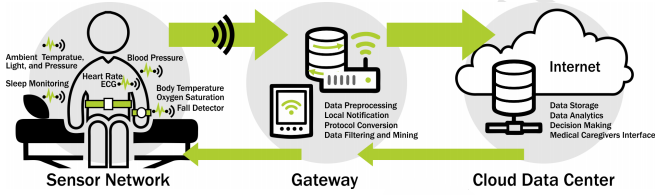
\includegraphics[scale=2]{figures/iotSetup.png}
     \caption{The position of the gateway in the current Internet infrastructure\cite{iotGatewaySlavesGraph}.}
     \label{fig:iotDeviceSetup}
 \end{figure}\\
But not everyone in the academic world was convinced that edge computing was indeed the way forward. 
However, establishing the need for edge computing is not the same as solving all problems though, and since then many papers have been published with titles such as "The Internet of Things Has a Gateway Problem"\cite{zachariah2015internetOfThingsHasGatewayProblem}. At the same time, researchers used custom IoT gateway solutions in their research and achieved impressive results. In one experiment, they achieved over 80\% performance increase in certain scenarios rightly titling their paper "From Cloud Computing to Fog Computing: Unleash the Power of Edge and End Devices"\cite{hong2017fromCloudtoIoTGatewayUnleashingTHePower}. Adding further to the problem of standardization is that IoT, especially IIoT, and mobile device have very different requirements.\\
This is the current place of the industry. There is a common agreement that fog computing is essential in the future, but no standard and open solution was developed yet. There is considerable effort in the academic world and in the industry to establish such a standard, one such initiatives is the Kubernetes IoT Edge working group under the Cloud Native Computing Foundry (CNCF). 




The space between the cloud and IoT and mobile devices, can be confusing at times. Knowing the history of IoT and the cloud is vital to understand the current developments. This, the methodology and the delimitation of this thesis will be discussed in the reminder of this section.\\




The terms used in the academic world and the industry are often different and many concepts partially overlap and complement each other making it hard to clearly categorize solutions. This is mainly due to ever evolving hard- and software, changing the possibilities of the devices and the entire landscape. It is thus imperative to clearly outline the key terms and design philosophies used of this thesis as well as presenting already existing solutions and how they compare to each other. These aspects are part of \cref{sec:eSOTA}, \nameref{sec:eSOTA}.\\
\Cref{sec:analysis}, \nameref{sec:analysis}, will lay the foundation to the actual implementation. We will motivate our design choices with academic and industry literature as well as with interviews from industry leaders. The focus of this thesis will be on the software and the requirements of the software to define and use the edge. Ultimately, it does not matter whether increases in performance and security come from better hardware or software, as long as the requirements are met. Consequently, the requirements will be ordered via the MoSCoW method. I will analyze the existing protocols, mainly for the application layer, and the data serialization method. Kubernetes is at the heart of this thesis implementation and extra sections will discuss what tricks Kubernetes already offers to control an edge cluster from the cloud and what might be missing. Additionally, I will look at extensions Kubernetes offers and how they could be useful in an IoT environemnt.\\


}

\comment{
The main focus is going to be on the software driving fog computing with an emphasize on IoT device and less mobile devices. 
We use a three tier layered network topology shown in \cref{fig:networkTopology3Layer}.
\begin{figure}[h!]
    \centering
    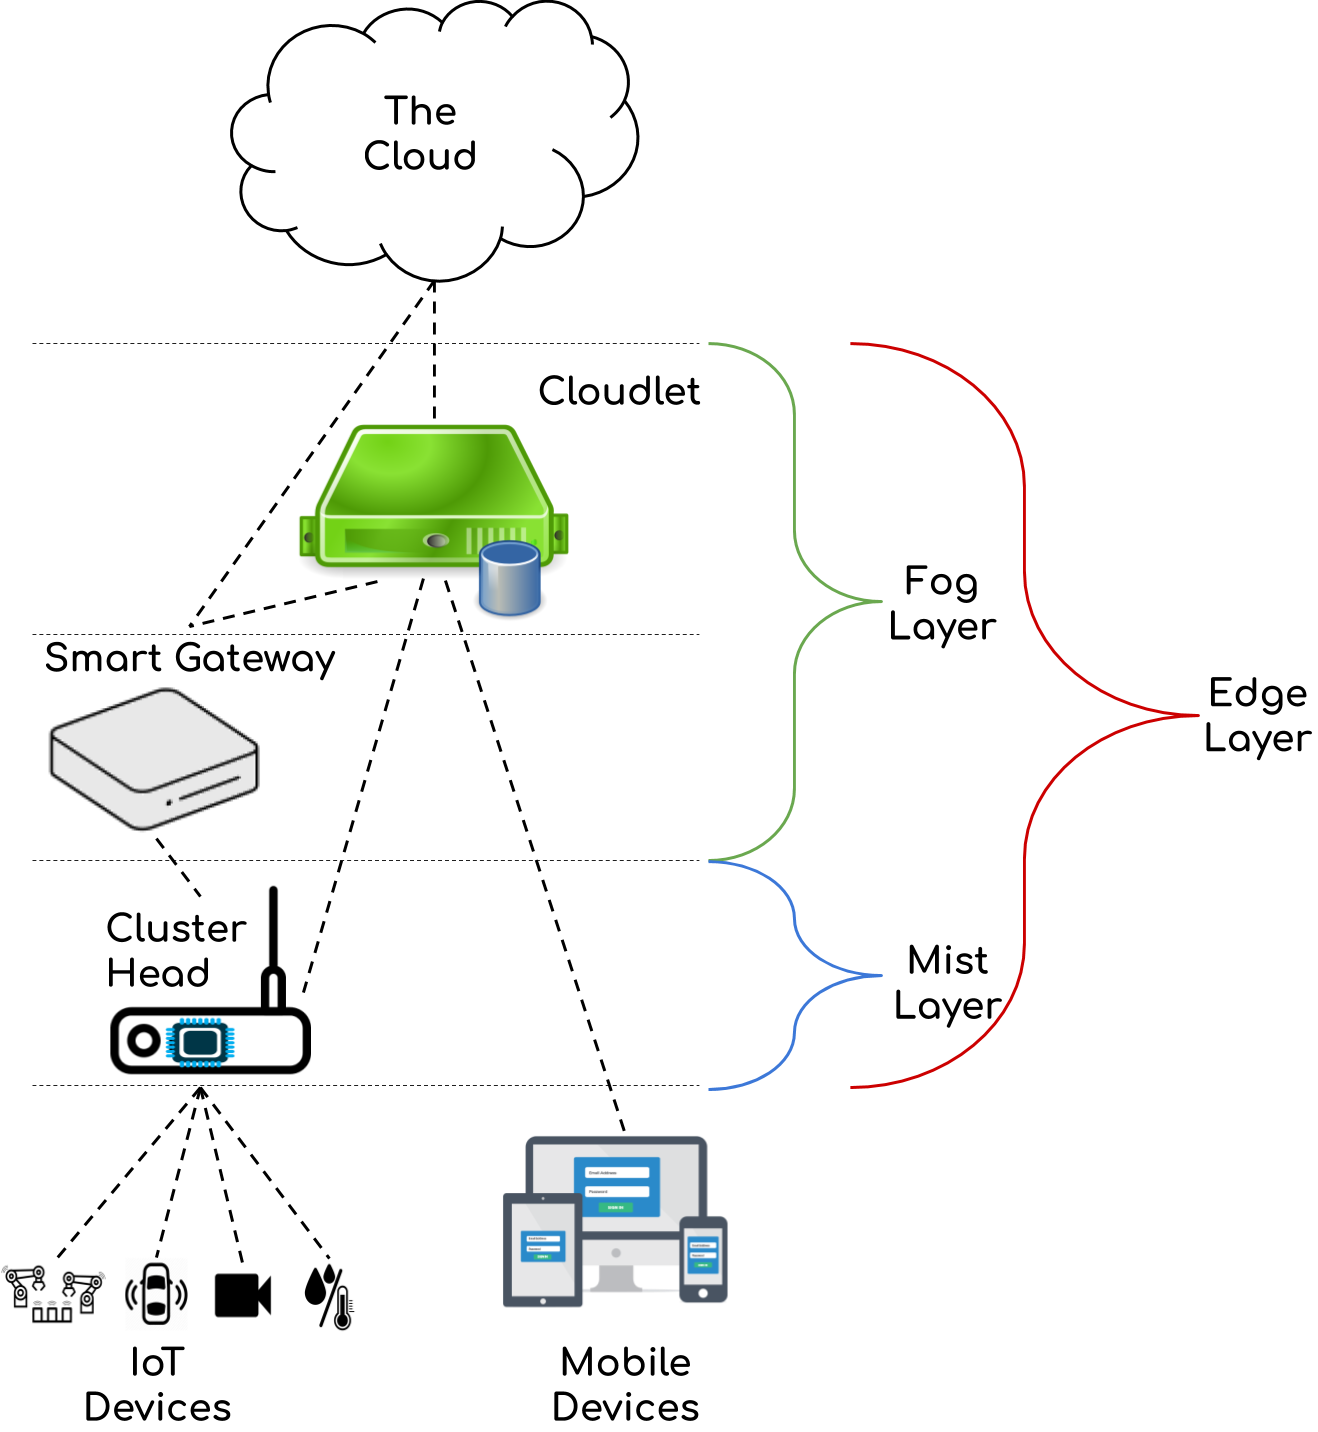
\includegraphics[scale=0.15]{figures/network-topology-3-layer.png}
    \caption{Three tier layer network topology, similar to \cite{nsa2017theNextWaveIoTDefinitions}}
    \label{fig:networkTopology3Layer}
\end{figure}
% Describe figure:
The cloud layer is made up of the 

% More detail
The cloud is the one layer where the authors think the technology stack is set. We expect Linux and Kubernetes, the de-facto standard for cloud orchestration, to be here to stay for the foreseeable future. This implies the same for x86\_64 and ARM, the only CPU architectures being supported by Linux. The Internets communication will remain in IPv4 and increasingly IPv6 for the Internet layer and TCP and UDP for the transport layer.\\ 
Quite the contrary is true for the bottom layer, IoT devices and mobile devices, although for the latter to a lesser extend. Communication in the IoT space is very diverse. Some protocols like 802.11 and Mobile

We expect IoT devices to have different software and different 
This can, but must not, include a control plane
The aim is to find the most promesing solution and 




Promesing solution with deep integration into K8s.


In essence, fog is the standard, and edge is the concept. Fog enables repeatable structure in the edge computing concept, so enterprises can push compute out of centralized systems or clouds for better and more scalable performance.
https://www.cisco.com/c/en/us/solutions/enterprise-networks/edge-computing.html


As it's name implies its aim is to develop an edge solution with Kubernetes support.

The need for smart IoT Gateways or fog computing is well established. They make it possible to 

Their design however is not. 
While the problems at the IoT edge — connectivity, manageability, scalability, reliability, security — are being solved as point solutions by enterprises and ecosystem players, there is a need for a foundational industry-wide standard for managing distributed IoT workloads.





IoT has seen a rapid growth over the last few years. According to IoT Analytics the total number of IoT devices is set to surpass the total number of other connected devices around 2021 \cite{StateofIoT:online}. Further, most IoT devices will be used in WPAN \footnote{Wireless Private Area Networks includes technologies like Zigbee,Z-wave and Bluteooth} and WLAN\footnote{Wireless Local Area Networks includes mainly Wi-Fi}. 
% In contrast to 5G, these technologies don't connect to an access point from an Internet provider but rather require another user operated device to connect to the Internet, a so called "gateway"


But fog computing does not come without its drawbacks. Depending on the protocol edge devices need to be close to their peers and slaves and physically accessible for maintenance. Which also poses a major security risk as they could be accessed by malicious intruders. The software maintenance is another critical aspects. Often IoT and edge devices are not update and patched with critical consequences. The "2016 Dyn cyberattack" used IoT devices like residential gateways, smart fridges, baby phones ect. to bring down the DNS-Servers operated by Dyn making large part of the Internet unaccessible for hours\cite{dynAttack}. The authors also stress that "large number of IoT devices are accessible over public Internet" and that "security (if considered at all) is often an afterthought in the architecture of many wide spread IoT devices"\cite{dynAttack}.\\
The question is then, how can manage and secure those devices. In this thesis, I will solely be concerned with the software aspect, which can mitigate some effects of exposing physical hardware to more accessible places.\\
Many challenges facing edge devices today have already been solved, although in a slight different context: The cloud\cite{IntroducingDejanBosanac:KubernetesIoTEdgeWorkingGroup}. In the cloud 




% Note: Maybe make a graph cloud setup, user connecting to nodes, VS fog computing, sensors and users connecting to gateways and gateway to cloud.  https://www.einfochips.com/blog/iot-gateways-drivers-for-fog-computing/

Kubernetes IoT Edge Working Group is a collaboration between Eclipse IoT Working Group and its 40-member companies, 35 open source projects, and Kubernetes ecosystem. It will define terminology, identify gaps in deployment and management, and educate the market on common use cases.
https://www.dailyhostnews.com/eclipse-foundation-and-cncf-working-together-to-bring-kubernetes-to-iot-edge
}
% \subsubsection{A Brief History}
\comment{
Why are IoT gateways important?
How did it come to be?
How did it start?
Why is it now, that many companies have interest?
}
Mobile devices profoundly changed the way computers interact with each other. Technopedia defines a mobile device as a "handheld tablet or other device that is made for portability, and is therefore both compact and lightweight"\cite{WhatisaM95TechnopediaMobileDevice:online}, it includes laptops, smartphones, tables etc. When these devices became a commodity in the 90s\footnote{Back then smartphones were called personal digital assistant (PDA).}, the way we manage computing power needed to change to accommodate intensive tasks on light weight computers. As Mahadev Satyanarayanan put it "while mobile elements will undoubtedly improve in absolute ability, they will always be at a relative disadvantage."\cite{satyanarayanan2015briefHistoryIoTGateway} Back then, researchers experimented with local, remote (cloud) and mixed execution also called adaptive
cloud offload. Assessing the three variants for voice recognition, video playback and web browsing locally, the researchers found huge gains from adaptive cloud offloading with a high enough bandwidth and concluded "the convergence of mobile computing and cloud computing enables new multimedia applications that are both resource-intensive and interaction-intensive."\cite{noble1997agileIoTGatewayOdyssey}. This lead to an explosion in cloud development. The Internet started out with a decentralized servers around the world. But over the years technologies were invented for orchestration across these distant servers, but also isolation for the local deployments. Probably the two main technological standards evolving where containers with containerd and orchestration with Kubernetes. \\
Traditionally, mobile devices connected to a gateway, which was mainly a router operating at L3\footnote{L3 stands for Layer 3, the networking layer in the OSI model.} to route packets and translate between different types of network protocols. \cite{lee2017futureOfIoT}. However, according to Dejan Bosanac, a senior software engineer at Red Hat in the field of cloud messaging and IoT platforms, due to their proximity to the sensors and the end user, these devices have three main advantages over the cloud: 
\begin{displayquote}
{\textbf{``Low latency, availability and locality''}}\cite{IntroducingDejanBosanac:KubernetesIoTEdgeWorkingGroup} - Dejan Bosanac.
\end{displayquote}
Because of these advantage researchers construct hybrid systems, in which devices operating on the edge of the network play an active role in the data processing pipeline. This architectural style of carrying out substantial amount of computation and storage at the edge is called "edge computing" \cite{fogComputing:def}. \Cref{fig:iotDeviceSetup} shows where the gateway is positioned in the current communication setup. 
 \begin{figure}[!h]
     \centering
     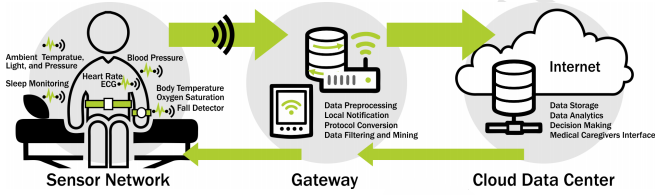
\includegraphics[scale=1.8]{figures/iotSetup.png}
     \caption{The position of the gateway in the current Internet infrastructure\cite{iotGatewaySlavesGraph}.}
     \label{fig:iotDeviceSetup}
 \end{figure}\\
But not everyone in the academic world was convinced that edge computing was indeed the way forward. In 2009, the National Science Foundation rejected a paper because \textit{``Many panelists do not agree with the premise of the proposal in which distant cloud computing incurs too high latency to be acceptable by mobile applications. They question the validity of such assumption as the proposal provides no real data to justify it[...]''}\cite{satyanarayanan2015briefHistoryIoTGateway}. Much has changed since then. The smartphone revolution (do I need to cite this? Is it a term I can actually use?) greatly increased the data produced by mobile devices and the need for speed and privacy. Researches did not foresee the explosion in IoT and the onset of a new wave data producers bundled under the term Indutrial IoT (IIoT). It includes hundreds and thousands of IoT devices working together, for example in factories, logistic warehouses, connected vehicles (CV), smart grid etc. In 2012 a widely cited paper "Fog Computing and Its Role in the Internet of Things"\cite{fogComputing:def} was published, establishing the need for IoT gateways connected to the cloud. The amount and high frequency of produced data is just too much to only handle in the cloud. Pre-processing on the edge is needed for both latency and efficiency.\\
However, establishing the need for edge computing is not the same as solving all problems though, and since then many papers have been published with titles such as "The Internet of Things Has a Gateway Problem"\cite{zachariah2015internetOfThingsHasGatewayProblem}. At the same time, researchers used custom IoT gateway solutions in their research and achieved impressive results. In one experiment, they achieved over 80\% performance increase in certain scenarios rightly titling their paper "From Cloud Computing to Fog Computing: Unleash the Power of Edge and End Devices"\cite{hong2017fromCloudtoIoTGatewayUnleashingTHePower}. Adding further to the problem of standardization is that IoT, especially IIoT, and mobile device have very different requirements.\\
This is the current place of the industry. There is a common agreement that fog computing is essential in the future, but no standard and open solution was developed yet. There is considerable effort in the academic world and in the industry to establish such a standard, one such initiatives is the Kubernetes IoT Edge working group under the Cloud Native Computing Foundry (CNCF). 


% \Cref{sec:problemArea}, \nameref{sec:problemArea}, will explain what challenges system designers face on the edge and why developing a standard is so hard.



























\subsection{Methodology}
The methodology describes the theoretical background for the methods applied in this thesis and ensures consistency across related work in the field.
The section Extended State of the Art is meant to provide the reader with an objective and complete overview of the research area. Following, in the Analysis section use cases are used to gather requirements. These are then prioritized according to the importance and feasibility for the desired system. Finally, in the Implementation, the system based on these requirements is implemented following a software development method and the priorities of the requirements.\\[5mm]
\textbf{\leftskip25mm\textit{Existing Solutions}}\\
The existing solutions section gives an objective presentations of already existing solutions in the field and sheds a light on how widely adopted systems or new once solve particular problems. It is not about the product but rather what the product tries to achieve and how.\\[5mm]
\textbf{\leftskip25mm\textit{Use Cases}}\\
Use cases are a way to find requirements\cite{UseCase94Fowler:online}. They can appear in the form of UML diagrams or written text. In this thesis only the written text version is used as the UML diagrams "[...]are of little value" and "the key value of use cases lies in the text" according to Martin Fowler\cite{UseCase94Fowler:online}. As the developed system is only a prototype I will use the "casual template for low-ceremony projects" from the book "Writing Effective Use Cases" from Alistair Cockburn\cite{cockburn2000writingUseCases}.\\[5mm]
\textbf{\leftskip25mm\textit{Functional Requirements}}\\
Functional Requirements state what services a system should provide, how it reacts to particular inputs, and how it should behave under particular circumstances\cite{sommerville2011software}. They are derived from the use cases and the state of the art and are the foundation for the implementation.\\[5mm]
\textbf{\leftskip25mm\textit{MoSCoW}}\\
The MoSCoW method is a way to structure the requirements according to the needs of the stakeholders involved\cite{sommerville2011software}. It is an acronym for "Must, Should, Could, Would". It helps to plan time and resources in a project so that the requirements with a higher ranking are finished first.\\[5mm]
\textbf{\leftskip25mm\textit{Agile Software Development Method}}\\
The software development method is a way to structure the development of software. An agile method emphasize development cycles to increase the transparency and flexibility during the software development. It decreases the risk of failure by constantly reevaluating the product. The agile manifest developed by industry experts\cite{beck2001manifestoAgile} has four main values: Individuals and Interactions over processes and tools; Working Software over comprehensive documentation; Customer Collaboration over contract negotiation; Responding to Change over following a plan. These are the foundation for a working agile software development method.

% \subsubsection{Delimitation} \label{sec:delimitation}
\comment{
Exclude hybrid cloud\\
Exclude non Kubernetes related technologies.\\
Exclude mobile devices.\\
Exclude hardware.\\
Exclude Sort of 5g and advances in mobile technologies.\\
Exlude infrastructure edge.\\
Exclude multi-cluster\\

}
